In the chapter 6 the dependence of the total  production cross-sections of intermediate mass fragments (from Be to Mg) in $p+Ag$ collisions at $Ep=480$ MeV on mass number A was discussed for different values of the third component of the izospin of fragments. 
This total cross-sections were model independent because they were extracted from integration of the experimental differential cross-sections $d\sigma/d\Omega dE$.  Furthermore the investigation of similar dependence was performed for model dependent production cross-section where the equilibrium processes of particle production were described by specific model, i.e. by GEMINI ++\cite{CHARITY1988,Charity2010} and the cross-sections for non-equilibrium processes were found as the difference between the experimental cross-sections and the GEMINI++ predictions.  

In the present chapter another investigation is presented of predictive power of the INCL++ model coupled to three models of the second stage of the process, i.e. GEMINI++, SMM\cite{SMMBondorf1995} and ABLA07\cite{kelic2009abla07}.  It was tested whether these model cross-sections are able
to reproduce very specific phenomenon observed in spallation reactions, namely the odd-even staggering of the total production cross-sections.
Odd-even staggering (OES) refers to the enhancement of production of odd Z particles to adjacent even- Z ones (or vice versa). Such an effect has been observed in many spallation and fragmentation reactions [72-76]. The main cause of this behavior is not yet fully understood, but it is usually attributed to phenomena related to the emission of particles from excited nuclei, in the context of pairing or mean-field effects (shell effects, nuclear deformations) that affect the density of nuclear states in the final step of the reaction processes. It has been observed that for neutron-deficient nuclei the OES effects are independent of the nuclear systems (projectile and target mass) and the beam energies\cite{Mei_OES}. However, this is not the case for isotopes of neutron-rich nuclei. Moreover, in the work of Ricchiardi et al \cite{RICCIARDI2004299_OES} it became clear that for the light fragments the OES effect is strong for the N = Z configuration and increases with the N-Z difference. Previous work suggested that the OES  and nuclear structure effects can be studied along the chain of the third component of the isospin (T$_3$ = (N-Z)/A), where such effects become prominent~\cite{Mei_OES}. In this work, the effects of OES are investigated using the IMF data measured by Green et al. \cite{Green1984} for which the total production cross-section for different IMFs was calculated in the previous chapter. The aim of this analysis is to examine the OES effects as a function of atomic number Z of the measured IMF for different values of T$_3$ and finally to compare the data with the predictions of INCL ++(v5.3) plus second stage models (SMM, ABLA07, GEMINI ++).
%
\section{Odd-Even staggering in total production cross-sections}
  It is interesting to compare the specific behaviour of total
  cross-sections as a function of Z.  It was shown on the basis
  of very rich set of fragmentation data published for $^{56}$Fe + p
  reaction at E/A=1 GeV that the total cross-sections reveal very characteristic dependence when presented as function of Z for individual values of T$_3$~\cite{napolitani2007measurement}. The cross-sections for even values of Z are systematically larger than those for odd values when nuclei with even (or odd) mass number A are taken into consideration.
  Such an effect, called odd-even staggering is
  strong for even-A nuclei and rather weak for odd-A nuclei.
  The staggering is most pronounced for
  T$_3$=0 (for even-A nuclei) and for T$_3$=-1/2 (for odd-A nuclei)
  decreasing when value of T$_3$ is significantly different from these values.
  As it was mentioned earlier that the
  procedure of determination of the total cross-sections applied in the present work is model
  independent.  Thus variation of the total cross-sections with
  changing A, Z and T$_3$ should correspond to the typical behaviour
  of the cross-sections observed in spallation and/or fragmentation
  of other target nuclei by energetic protons. This is indeed the
  case as can be seen in Fig.~\ref{fig:TOTG23staggering} (present work). 
  %\begin{figure*}
\begin{figure}[!h]
  % Requires \usepackage{graphicx}
  \centering
  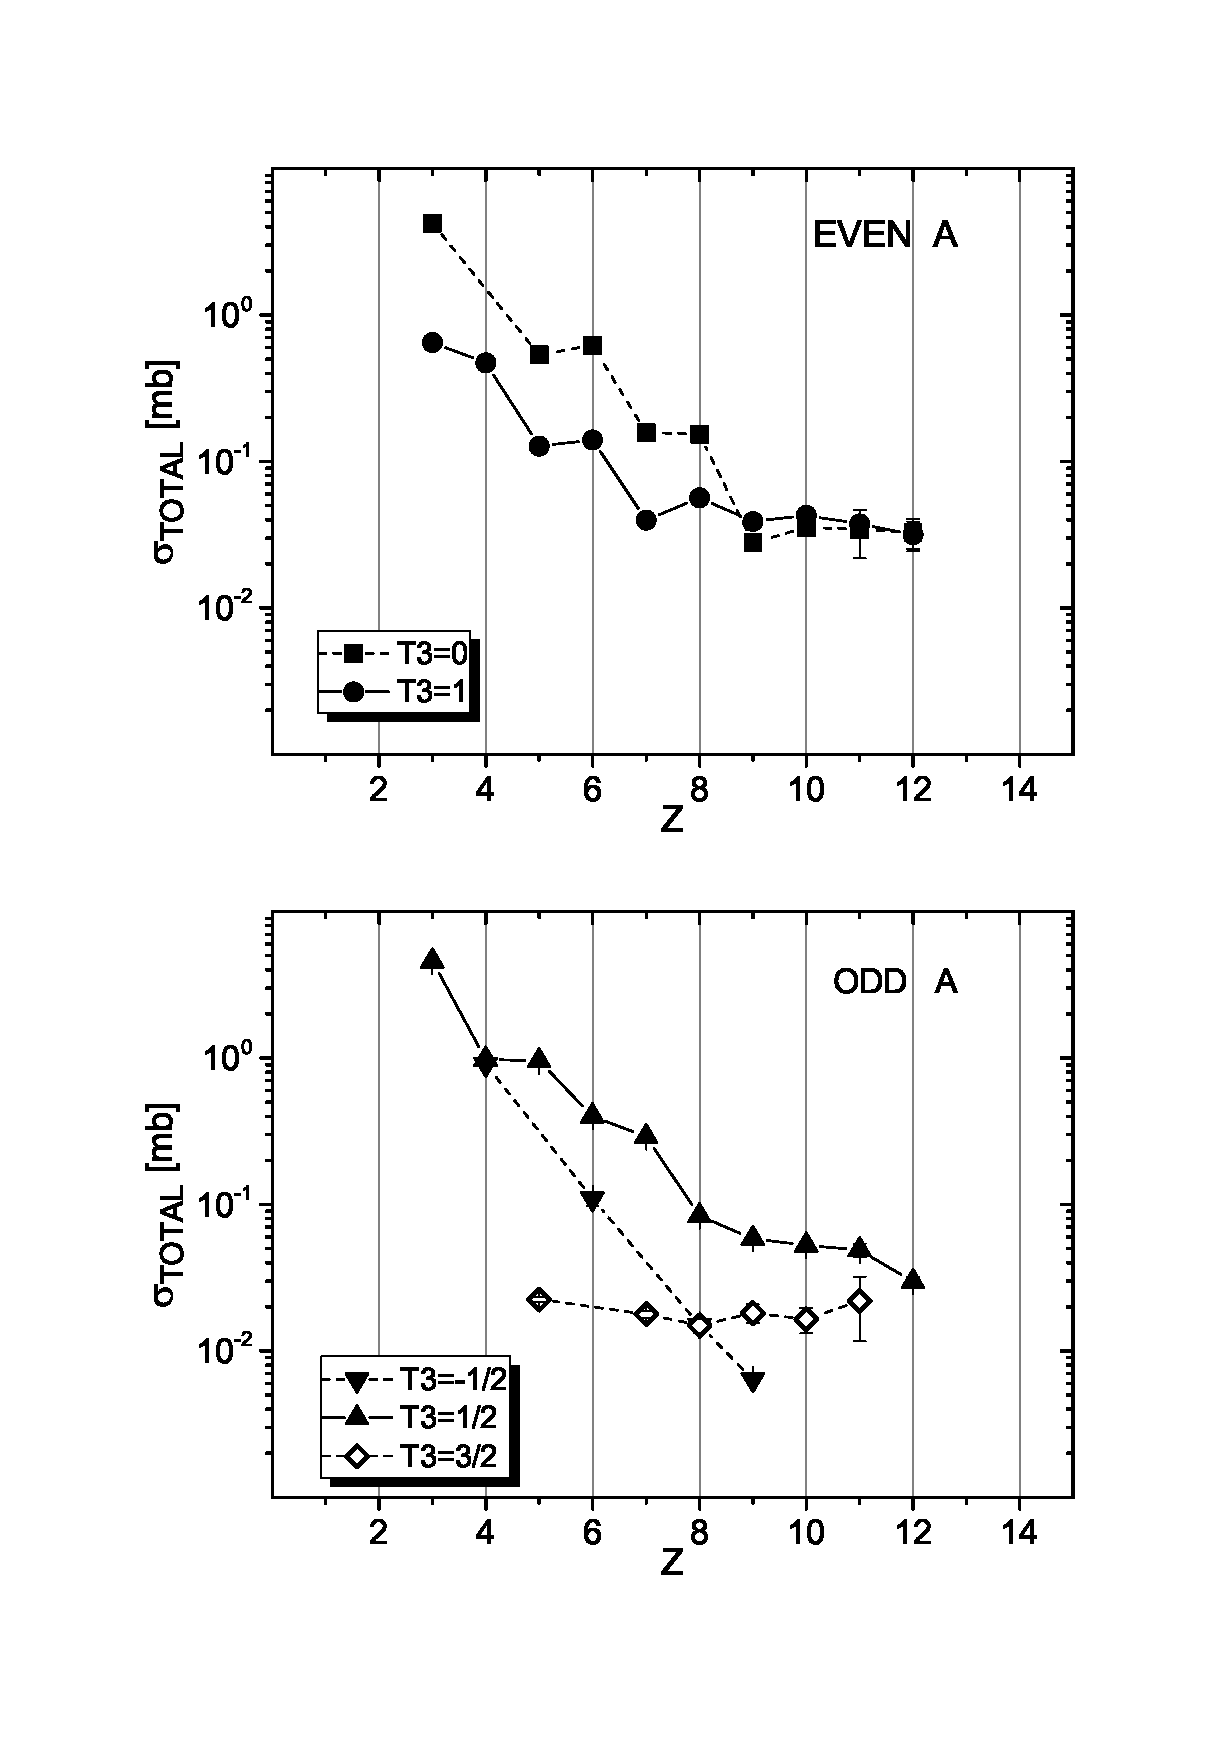
\includegraphics[width=0.84\textwidth]{TOTG23staggering.eps}
  \caption{The atomic number Z dependence of total production cross-sections
  for even-mass nuclei (left panel of the figure) and for odd-mass nuclei (right panel).
  cross-sections representing intermediate mass fragments with the same third component
  of the isospin $T_3 \equiv (N-Z)/A$
  are shown by the same symbols connected by thin lines.
  }
  \label{fig:TOTG23staggering}
\end{figure}
%\end{figure*}
%
  Odd-even staggering of the total cross-sections is pronounced for even-A nuclei and is  not visible for odd-A
  nuclei (Fig.~\ref{fig:TOTG23staggering}).
  Therefore, it is concluded that the total cross-sections dependence
  on A, Z and T$_3$ found in the present investigation agrees qualitatively with typical behaviour of
  spallation and fragmentation data. 
To quantitatively discuss the staggering effect of the data and compare it with the predictions of the models, one needs to introduce a variable ($\delta$) whose value would provide the needed information. This is discussed in the next section.
%
\section{Dependence of $\delta$ on third component of isospin}\label{quanti_theory}
To quantify OES effect, a procedure proposed by Tracy \emph{et al.} \cite{TRA72A} was applied in the form given by Ricciardi \emph{et al.}~\cite{RICCIARDI2004299_OES} for the Z-dependence of cross-sections at a fixed N-Z. The $\delta$  value greater than zero (less than zero) evaluated by Equation \ref{eq:delta} gives a relative increase in the cross-section for even-Z (odd- Z) products with respect to a smooth Z dependence.

\begin{equation}\label{eq:delta}
\delta \left( {Z + 3/2} \right) \equiv \frac{1}{8}\left( { - 1}
\right)^{Z + 1} \left[ {\left( {L_3  - L_0 } \right) - 3\left( {L_2
- L_1 } \right)} \right]
\end{equation}
%
where

\[
L_i \equiv  ln (\sigma\left( Z+i \right))
\]
%
The $\delta$ value is assigned on the midpoint of the Z interval from Z to Z+3 where smooth Z-dependence was postulated.
The $\delta$-function values are shown in Fig.~\ref{Fig:Deltavsz} for experimental total cross-sections (open black squares) and for theoretical cross-sections (solid colored symbols). The theoretical cross-sections were evaluated using INCL++ as the first-stage model and three different second-stage models (ABLA07, GEMINI++ and SMM) describing the de-excitation of the equilibrated, excited residual nucleus from the intranuclear cascade. 
%
\begin{figure}[!h]
\centering
\includegraphics[width=0.95\textwidth]{Delta.eps}
\caption{Plot of the $\delta$-function versus atomic number Z of the
reaction products. The open, black squares depict values of the
$\delta$-function evaluated for experimental cross-sections whereas
magenta, green, and red symbols correspond to the $\delta$-function
values obtained with the cross-sections of ABLA07, GEMINI++ and SMM
models, respectively.} \label{Fig:Deltavsz}
\end{figure}
As in Fig. \ref{Fig:Deltavsz}, the delta function values are positive for the cross-sections of IMF with N=Z (upper left panel of the figure) and N=Z+2
(lower left panel) obtained from experimental data. In contrast, the delta function is negative for
IMF with N=Z+1 (upper right panel ) and N=Z+3 (lower right panel ). This indicates that the even Z cross-sections for N=Z and N=Z+2 are larger than the smooth trend, while it is the case of the odd- Z cross-sections for N=Z+1 and Z+3. This information is in perfect agreement with the qualitative conclusions drawn from the inspection of Fig. \ref{fig:TOTG23staggering}, where the experimental cross-sections are collected.

Moreover, the absolute values of the $\delta$ function are close to zero for the products with N=Z+3, while they are drastically different from zero for other products. This information is again consistent with Fig. \ref{fig:TOTG23staggering}, where the Z-dependence of the cross-section is lowest for N=Z+3 (smooth line), especially compared to N=Z and N=Z+2 (zigzag line). Moreover, the values of the $\delta$-functions for the experimental cross-sections approach zero as the atomic number Z of the products increases, which is consistent with the general trend that the OES effect decreases with increasing Z (cf. Ref.~\cite{Mei_OES}).

Despite the general agreement between the sign of the $\delta$-function of the experimental cross-sections and those of all three models, there are also visible discrepancies between experimental and theoretical $\delta$-functions. They are particularly clear for products with N=Z+2. In this case, the $\delta$-function evaluated for experimental cross-sections \emph{decreases} from values around 0.3 at
Z=4.5 to zero at Z=10.5, while the $\delta$-function determined for the GEMINI ++
cross-sections \emph{increases} monotonically from -0.05 at Z=4.5 to 0.47 at Z=10.5.
Thus, the tendency of the variation of the experimental $\delta$-function and that of GEMINI ++ is also not reproduced.
%%%%%%
There are clear differences between the experimental and model $\delta$-function for
ABLA07 (the $\delta$-function values do not change monotonically) and for SMM
(the $\delta$-function values are large and positive for only two points in the interval 4.5 - 10.5, while they are small and negative at both ends of this interval).
Smaller but also significant differences between experimental and model $\delta$-function exist for reaction products with N = Z. The shape of all model
$\delta$- function is almost the same as that of the experimental $\delta$- function, but there are two differences. The magnitude of the experimental and model $\delta$-function values are different, and the position of the maximum of the model $\delta$-function is different from that of the experimental one.

The question arises as to the origin of the differences between the $\delta$-
function obtained from the experimental cross-sections and that calculated from model cross-sections applied in the framework of the two-stage model with different models describing the second stage of the reaction. The natural candidate for explaining these differences seems to be the neglect of non-equilibrium processes in the model calculations. They were introduced in a phenomenological way in the overall experimental cross-sections but are not explicitly present in the model cross-sections. They are only included in the evaluation of the cross-sections of light charged particles, which are not analyzed in the present study. Of course, they affect the population of residual nuclei after the intranuclear cascade due to the coalescence of nucleons into ejectiles consisting of less than 5 nucleons. Moreover, such a coalescence process changes the population of excited states of the residual nuclei of the cascade.
To check whether an increase in the coalescence of nucleons during the stage of the intranuclear cascade can significantly modify the $\delta$- function determined from model cross-sections, we repeated the model calculations and extended the coalescence effect to intermediate-mass fragments with mass number A equal to 8. It was found that such a modification has no significant effect.
%
%\section{Summary}

%In this chapter the OES, \emph{i.e.} the effect of the
%staggering in the yields of intermediate mass fragments produced in
%p+Ag collisions at proton beam energy of 480 MeV has been studied.
%Since the total production cross-sections were not measured for this
%reaction they were determined by integration of the experimental
%double differential cross-sections d$^{2}\sigma$/d$\Omega$dE of Ref.
%\cite{Green1984}. These double differential cross-sections were
%analyzed by combination of the two-step model of the intranuclear
%cascade INCL++ followed by the de-excitation of the equilibrated
%remnant nucleus of the cascade in the frame of the GEMINI++ model.
%The difference between predictions of this model and the
%experimental data were fitted by means of the phenomenological model
%of one or two isotropically emitting sources moving forward (along
%the beam direction).  Such a method provided model independent
%values of the experimental cross-sections because combination of the
%above models can be treated as a mean for appropriate interpolation
%and extrapolation of the data for full angular and energy range
%available.
%
%The obtained total cross-sections were analyzed qualitatively as a
%function of atomic number Z of the products as well as
%quantitatively by application of the $\delta$-function proposed by
%Tracy \emph{et al.} \cite{TRA72A} for determination of the relative
%enhancement of the cross-sections for even-Z (odd-Z) products in
%respect to their smooth Z dependence. It was found that a
%significant OES effect is present, most pronounced for products with
%N=Z, N=Z+1 and N=Z+2.  In the first and the third case the even-Z
%products are produced with relatively larger cross-sections in
%respect to the smooth Z-dependence whereas in the second case this
%was true for odd-Z products.
%
%The staggering of the experimental total cross-sections were
%compared with that observed for the theoretical cross-sections of
%two step model. The first stage of the reaction was described by
%INCL++ model with inclusion of coalescence of escaping nucleons from
%the intranuclear cascade into complex nuclei with mass number A
%smaller than 5 and, separately, with mass number A smaller than 9.
%In both cases the second stage of the process, \emph{i.e.} the
%de-excitation of the equilibrated nucleus remnant of the
%intranuclear cascade was modeled by three different programs:
%ABLA07, GEMINI++ and SMM.  It was found that the main properties of
%the experimental cross-section staggering, \emph{i.e.} the sign of
%the $\delta$-function as well as its average value was reproduced by
%all three models.  However, quite significant differences appeared
%as concerns details of the staggering, i.e. the shape of the
%Z-dependence of the $\delta$-function and to smaller extent its
%values.  The strongest differences were observed for N=Z+2 nuclei.
%
%While the origin of the difference between the data and model
%predictions may be attributed to the lack of knowledge of
%non-equilibrium processes which seem to be quite important for the
%studied reactions  the significant difference between predictions of
%various theoretical models is not understood.
%%
%Present results indicate that the OES seems to be a demanding effect
%for testing the assumptions  underlying different theoretical models
%of the spallation reactions and therefore its investigation may be
%helpful in their development.
